\documentclass[a4paper,12pt]{report}

\usepackage[margin=1in]{geometry} % Set margins

\renewcommand{\baselinestretch}{1.5} % Set line spacing

\usepackage{times} % Set font to Times New Roman

\usepackage{graphicx} % Images

\setlength{\parindent}{0pt} % Paragraph indentation to start from start.

\usepackage{hyperref} % For Links

\usepackage{listings} % For python code
\usepackage{xcolor}

\definecolor{codegreen}{rgb}{0,0.6,0}
\definecolor{codegray}{rgb}{0.5,0.5,0.5}
\definecolor{codepurple}{rgb}{0.58,0,0.82}
\definecolor{backcolour}{rgb}{0.95,0.95,0.92}

\lstset{
    language=Python,
    basicstyle=\ttfamily\small,
    numbers=left,
    numberstyle=\tiny\color{codegray},
    frame=single,
    backgroundcolor=\color{backcolour},
    commentstyle=\color{codegreen},
    keywordstyle=\color{blue},
    numberstyle=\tiny\color{codegray},
    stringstyle=\color{codepurple},
    breaklines=true,
    breakatwhitespace=true,
    captionpos=b,
    showstringspaces=false,
}

\usepackage{booktabs} % for csv
\usepackage{longtable}

\begin{document}

% Cover page
\begin{titlepage}
    \centering
    {\Huge\bfseries FLOOD FORECASTING USING MACHINE LEARNING \par}
    \vspace{1.3cm}
    
    {\Large Submitted By \par}
    {\Large \textbf{Saurabh Tiwari (2020CE10295)} \par}
    \vspace{1.3cm}
    
    {\Large Supervised by \par}
    {\Large \textbf{Prof A.K. Keshari} \par}
    \vspace{1.3cm}

     {\Large A report of CVD411 - Project Part 1 submitted 
    in partial fulfillment of the requirements of the degree of 
    Bachelor of Technology \par}
    \vspace{1.9cm}
    
    
\includegraphics[width=0.3\textwidth]{iitd-logo.png} % IITD logo image
    
    {\Large Department of Civil Engineering \par}
    {\Large Indian Institute of Technology Delhi \par}
    {\Large November, 2023 \par}
\end{titlepage}

% Preliminary pages with roman page numbering
\pagenumbering{roman}

% Certificate Student and Prof
\chapter*{\centering \underline{CERTIFICATE}}

\addcontentsline{toc}{section}{Certificate}

I do certify that this report explains the work carried out by me in the Course CVD411 - Project Part 1 under the overall supervision of \textbf{Prof A.K. Keshari}. The contents of the report including text, figures, tables, 
computer programs, etc. have not been reproduced from other sources such as books, journals, reports, manuals, websites, etc. Wherever limited reproduction from another source had been made, the source had been duly acknowledged at that point and also listed in the References.

\vspace{2cm}

\begin{raggedleft}

\textbf{Saurabh Tiwari} \\
\today

\end{raggedleft}

\vspace{2cm}

This is to certify that the report submitted by \textbf{Saurabh Tiwari} describes the work carried out by him in the Course CVD411 - Project Part 1 under my overall supervision.

\vspace{2cm}

\begin{raggedleft}

\textbf{Prof A.K. Keshari} \\
Professor, Department of Civil Engineering \\
Indian Institute of Technology Delhi \\
\today

\end{raggedleft}


% Acknowledgment
\chapter*{\centering \underline{ACKNOWLEDGMENT}}

\addcontentsline{toc}{section}{Acknowledgement}

I would like to express my sincere gratitude to my supervisor, \textbf{Prof A.K. Keshari}, for his guidance, support, and valuable feedback throughout the course of this project. His expertise and insights have been invaluable in shaping this work. I am also thankful to the \textbf{Department of Civil Engineering, Indian Institute of Technology Delhi}, for providing the necessary resources for the completion of this project.

\vspace{2cm}

\begin{raggedleft}

\textbf{Saurabh Tiwari} \\
\today

\end{raggedleft}


% Abstract
\chapter*{\centering \underline{ABSTRACT}}

\addcontentsline{toc}{section}{Abstract}

This report presents a novel approach to flood prediction and mitigation, specifically tailored for the challenging context of the Indian Subcontinent. Recognizing the devastating impact of floods on communities, the project addresses the scarcity of comprehensive data in India by pioneering the extraction of information from local news reports, creating a robust dataset that sets it apart from traditional flood forecasting models.

Motivated by the urgent need to address the pervasive and severe impact of floods in India, the project develops a proactive tool for predicting and visualizing potential flood scenarios before they occur. By synthesizing complex data into an interactive and comprehensible format, the web application named "Flood Predictor" empowers individuals and governments to make informed decisions in the face of imminent threats.

The project's significance is rooted in the alarming statistics surrounding flood-related disasters in India, with over 80\% of the population at risk. Beyond the immediate threat to life and property, floods exert a profound socioeconomic toll, contributing to an annual economic loss of nearly 15 billion USD in India alone. In response to this imperative, the Flood Predictor application emerges as a cost-effective and accessible solution, facilitating equitable distribution of resources and minimizing the impact of floods on vulnerable communities.

The objectives of the project include innovative data collection methods, implementation and optimization of a cutting-edge machine learning model, advanced data visualization techniques, and the development of an intuitive web application. The machine learning model, based on the Random Forest Classifier, achieves an impressive accuracy of 98.71\% on the test set. The web application, hosted on AWS Elastic Beanstalk, provides real-time flood predictions for any city in India, contributing to proactive measures and informed decision-making.

The report concludes with a reflection on the journey, acknowledging the challenges overcome, and outlines future directions for expanding the application globally and incorporating satellite data for enhanced flood detection. The Flood Predictor project stands as a technological achievement with the potential to make a significant impact on flood preparedness and resource allocation, showcasing the possibilities of leveraging technology for the greater good.


\tableofcontents


\listoffigures  % Generate the list of figures

\addcontentsline{toc}{section}{List of figures}

\listoftables  % Generate the list of tables

\addcontentsline{toc}{section}{List of tables}


\chapter{Introduction}

% Main sections with arabic page numbering
\pagenumbering{arabic}

\section{General}

Floods, as one of the most devastating natural disasters, pose a significant threat to communities worldwide, necessitating innovative approaches to prediction and mitigation. While flood forecasting models abound, the uniqueness of this report lies in its original methodology, particularly tailored for the challenging context of the Indian Subcontinent.

\vspace{0.5cm}

\begin{figure}[ht]
  \centering
  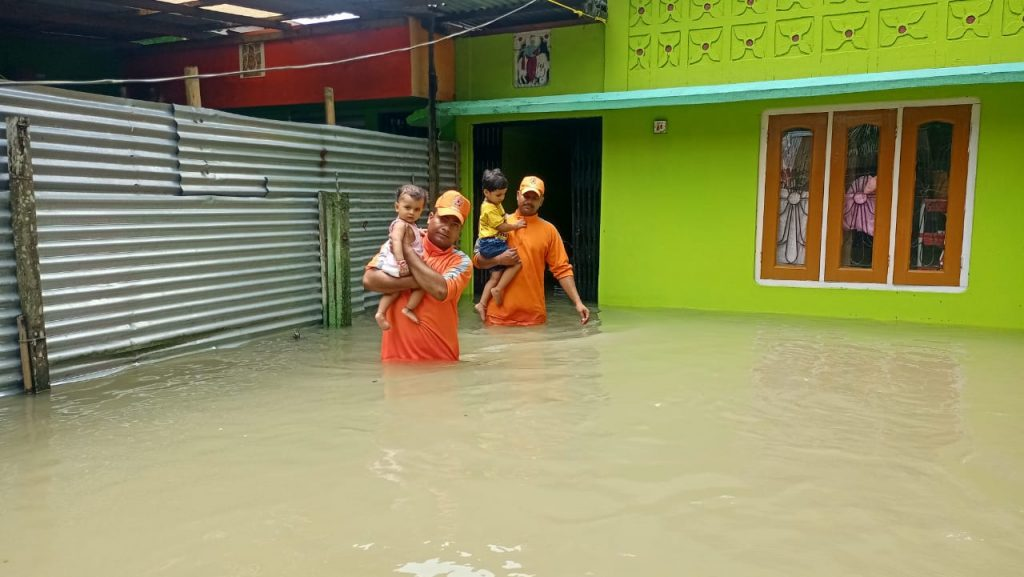
\includegraphics[width=\linewidth]{Flood-Introduction.jpeg}
  \caption{Flood rescue in Assam, India, June 2022 – NDRF}
\end{figure}


\section{Uniqueness}

Unlike regions like the United States, where abundant flood-related data simplifies predictive modeling, the scarcity of comprehensive data in India prompted the development of an unconventional approach. Rather than relying on satellite imagery, my project pioneers the extraction of information from local news reports. This involves mining data on flood occurrences, discerning location and time frames, and subsequently collating relevant weather conditions such as temperature, wind speed, cloud cover, humidity, and precipitation. This novel approach distinguishes my project, providing a robust dataset that sets it apart from traditional flood forecasting models.

\section{Significance}

Motivated by the urgent need to address the pervasive and severe impact of floods, the significance for my project is rooted in the alarming statistics surrounding flood-related disasters in India. With over 80\% of the population, approximately 1.08 billion people, at risk, and recent calamities like the Kerala flood tragedy claiming lives and destroying homes, the imperative for proactive flood prediction becomes evident. Coupled with the escalating risks attributed to climate change, the frequency and intensity of floods demand innovative solutions to mitigate their devastating consequences.

In response to this imperative, my project emerges as a proactive tool aimed at predicting and visualizing potential flood scenarios before they occur. By synthesizing complex data into an interactive and comprehensible format, the application empowers both individuals and governments to make informed decisions in the face of imminent threats.

\section{Socioeconomic Cause}

Beyond the immediate threat to life and property, floods exert a profound socioeconomic toll. Globally, floods contribute to an annual economic loss of nearly 40 billion USD, with India alone accounting for 15 billion USD per year. Recognizing the critical role of preventive measures in mitigating these losses, my project endeavors to bridge the resource gap. By offering a cost-effective and accessible solution to governments and citizens alike, the application aims to facilitate equitable distribution of resources, thus minimizing the impact of floods on vulnerable communities. In essence, my project aligns with the principle that proactive intervention can be a powerful force in averting the devastating consequences of floods and fostering societal resilience.


\chapter{Objective}

\section{Data Collection}
The primary objective is to introduce an innovative approach to data collection for flood prediction, particularly in the challenging context of the Indian Subcontinent. This involves pioneering a methodology that taps into local news reports to extract crucial information about flood occurrences. The uniqueness of this approach lies in its fusion with historical weather conditions, overcoming the scarcity of comprehensive flood-related datasets in the region. The goal is to establish a robust and contextually rich dataset that enhances the accuracy and specificity of flood predictions.

\section{Machine Learning Model}
The core focus is on implementing and optimizing a cutting-edge machine learning model. The objective is to achieve a high level of accuracy through an exhaustive process of model experimentation. This includes testing various machine learning models, from Logistic Regression to K-Nearest Neighbors. The aim is to contribute to the advancement of machine learning applications in the domain of natural disaster prediction.

\section{Data Visualization}
The objective is to employ advanced data visualization techniques to enhance the interpretability and accessibility of flood-related insights. Utilizing the Plotly chart studio, the focus is on creating dynamic and interactive visualizations such as bubble plots and density maps. These visualizations play a pivotal role in conveying complex information in an easily understandable format, facilitating effective communication of flood predictions, damage estimates, and precipitation analyses to both experts and the general public.

\section{Web Application Development} 
A key objective is the development of an intuitive and user-friendly web application, named "Flood Predictor." Built on the Flask Python framework, the application seamlessly integrates the machine learning model, datasets, and visualizations. By allowing users to input the name of a city, the application fetches real-time weather forecast data, runs it through the machine learning model, and presents instantaneous flood predictions. The goal is to make flood-related information easily accessible to a broad audience, including government officials, researchers, and the general public, thereby promoting proactive measures and informed decision-making.


\chapter{Literture Review}

\section{Ambore, Charan, et al. (2023)}
The authors presents an examination of diverse machine learning algorithms for predicting floods based on rainfall data in Indian districts. Previous works on flood prediction using techniques like support vector machines, neural networks, image processing, and big data analytics are reviewed. The employed machine learning algorithms in this study include XGBoost, K Nearest Neighbors, Decision Trees, Logistic Regression, and Random Forest. Performance metrics such as accuracy, precision, recall, and F1-score are used to demonstrate the effectiveness of the models. A comparison with existing methods is conducted, and the advantages and limitations of the approach are discussed.

\section{Mosavi, Ozturk, et al. (2018)}
The report presents the challenges and importance of flood prediction for risk reduction and water resource management. The advantages and disadvantages of different types of models, such as physically based, statistical, and data-driven models. The state of the art of machine learning methods, such as artificial neural networks, support vector machines, decision trees, and ensemble methods, for both short-term and long-term flood prediction. The performance comparison and evaluation of various machine learning models based on accuracy, robustness, generalization, and computation cost. The trends and future directions of improving machine learning models, such as hybridization, data decomposition, algorithm ensemble, and model optimization.

\section{Xiong \& O'Connor (2002)}
The author presents a comparison of four updating models for real-time river flow forecasting, based on the simulation errors of a rainfall-runoff model. The four models are:
\begin{enumerate}
\item Single autoregressive (AR) model: the most widely used model, which fits a linear regression to the error series.
\item Autoregressive-threshold (AR-TS) model: a model that divides the error series into different bands according to the flow magnitude, and fits a separate AR model for each band.
\item Fuzzy autoregressive-threshold (FU-AR-TS) model: a model that uses fuzzy logic to assign different degrees of membership to the error values for each band, and combines the outputs of the AR models using weighted averages.
\item Artificial neural network (ANN) model: a model that uses a three-layer feed-forward network to capture the nonlinear relationship in the error series.
\end{enumerate}
The author applies these four models to 11 test catchments, using the soil moisture accounting and routing (SMAR) model as the substantive rainfall-runoff model. The author evaluates the performance of the models using the Nash-Sutcliffe efficiency index and other criteria. The author finds that all four models can improve the flow forecast accuracy over the nonupdating mode, but the AR-TS, FU-AR-TS, and ANN models do not show significant advantages over the simple AR model. The author recommends the use of the AR model for error-forecast updating in real-time river flow forecasting.

\section{Nevo, Morin et al. (2018)}
The report talks about:
\begin{enumerate}
\item Flood forecasting with machine learning: Google's operational flood warning system uses machine learning models to provide accurate and timely alerts to agencies and the public in India and Bangladesh. The system consists of four subsystems: data validation, stage forecasting, inundation modeling, and alert distribution.
\item Stage forecast models: The system uses two types of models to predict future river stages at target gauges: a Linear model based on multiple linear regression, and a LSTM model based on a recurrent neural network. The LSTM model showed higher skills than the Linear model in most cases.
\item Inundation models: The system uses two types of models to map flood extent and depth from forecasted river stages: a Thresholding model that does not require a digital elevation model (DEM), and a Manifold model that does require a DEM and also computes inundation depth. The Manifold model is a novel machine-learning alternative to hydraulic models. The Thresholding and Manifold models achieved similar performance metrics for modeling inundation extent.
\item Alerts: The system disseminates flood alerts to relevant agencies and the public via different channels, such as Google Search, smartphone notifications, and Google Maps. The alerts include information about the forecasted water stage, the inundation map, and the inundation depth if available. The alerts are sent in the local language and are designed to be informative and actionable.
\end{enumerate}


\chapter{Methodology}

\section{Data Collection}

\subsection{Web Scraping}

In the initial phase of data collection, the Python Beautiful Soup 4 library was employed to perform web scraping on the designated website, http://floodlist.com/tag/india. This process involved the systematic extraction of flood-related data encompassing both historical and current events. The extracted information included crucial details such as the dates and geographical locations of the reported floods. By leveraging this web scraping technique, a foundational dataset was established to form the basis for subsequent analyses.

\subsection{Weather API}

The utilization of the Visual Crossing Weather API constituted a pivotal aspect of the data collection process. This API was instrumental in retrieving comprehensive historical weather data for areas affected by floods. The specific weather parameters obtained included precipitation levels, humidity, temperature, cloud cover, and wind speed. This dual approach of combining web scraping with data from the Weather API ensured a holistic and nuanced dataset, incorporating both flood-specific and meteorological information.

\subsection{Data Augmentation}

To enhance the richness and diversity of the dataset, various data augmentation techniques were systematically applied. These techniques were employed to synthetically increase the volume of training data without necessitating the collection of entirely new information. By incorporating augmentation strategies, the dataset's robustness and representativeness were substantially improved, contributing to the overall efficacy of the machine learning model.

\section{Machine Learning Model}

My machine learning model is based on the python sci-kit learn library. A thorough exploration of multiple machine learning models, including Logistic Regression, K-Nearest Neighbors, and Random Forest Classification, was conducted. Subsequently, the trained model was preserved in a pickle file, setting the stage for seamless integration into the web application.

\section{Data Visualization}

I first obtained a dataset of the major cities and towns in India (around 200 of them) along with their latitude, longitude, and population. I then obtained the numerous weather factors in each city using the weather API and ran the data into my machine learning model. Next, I plotted the data from the model on various different types of maps, using Plotly chart studio.

The development of data visualizations comprised three fundamental components: Scatter Plots, Bubble Plot and Density Maps. Plots provided insights into flood predictions, damage predictions, and heavy rainfall predictions through visually intuitive representations. Density maps, on the other hand, employed color gradients to convey the magnitude of flood-related metrics.

\section{Web Application Development}

\subsection{Frontend}
The web application was implemented using the Flask Python framework, leveraging its capabilities for seamless integration with machine learning models. The presentation layer incorporated HTML templates for structure, CSS for styling, and Javascript to enhance the user experience and functionality.
On my predict page, the user simply enters the name of any city in India. My app then automatically fetches the weather forecast data of that city in realtime, runs this data into my Machine Learning model, and gives instantaneous results, which include the flood prediction, the temperature, the maximum temperature, the humidity, the cloud cover, the windspeed, and the precipitation.

\subsection{Integration and Hosting}
The integration phase involved the seamless connection of the Flask back-end with the developed machine learning models and datasets. To make the web application accessible to a wider audience, AWS Elastic Beanstalk was utilized for hosting, ensuring scalability and reliability in serving the application to users. This robust integration framework laid the foundation for the successful deployment and utilization of the Flood Predictor web application.

\chapter{Results}

\section{Final data required for ML training}

\begin{table}[ht]
\centering
\begin{center}
\begin{longtable}{cccccccc}
\toprule
\textbf{Temp} & \textbf{Max\_Temp} & \textbf{Wind\_Speed} & \textbf{Cloudcover} & \textbf{Precip} & \textbf{Humidity} & \textbf{Class} \\
\midrule
29.90 & 37.00 & 23.00 & 58.60 & 146.00 & 83.86 & 1 \\
93.04 & 82.41 & 63.44 & 102.42 & 192.07 & 129.30 & 1 \\
87.13 & 98.82 & 72.29 & 122.12 & 191.80 & 142.25 & 1 \\
92.12 & 72.39 & 73.84 & 96.50 & 196.53 & 150.42 & 1 \\
92.64 & 76.03 & 67.13 & 92.61 & 191.76 & 126.61 & 1 \\
\multicolumn{7}{c}{...} \\
61.43 & 77.45 & 80.24 & 77.38 & 81.32 & 124.24 & 0 \\
72.26 & 78.98 & 47.48 & 73.92 & 67.72 & 113.09 & 0 \\
76.40 & 82.69 & 79.23 & 58.95 & 65.84 & 122.76 & 0 \\
61.03 & 74.17 & 70.44 & 61.39 & 64.09 & 106.96 & 0 \\
85.19 & 64.06 & 73.84 & 56.96 & 71.45 & 109.65 & 0 \\
\bottomrule
\end{longtable}
\small\textit{[5040 rows x 7 columns]}
\end{center}
\caption{Final data required for ML training}
\end{table}

The Python code to generate this data can be found in Section 8.1

A binary classification system is utilized in the "Class" column, where the label "1" indicates the presence of a flood, while "0" signifies the absence of a flood.

\section{Machine Learning Model Accuracy}

The parameters employed in the machine learning model include temperature, max temperature, wind speed, cloud cover, humidity, and precipitation. Following extensive experimentation with various models, the Random Forest Classifier yielded the highest accuracy of 98.71\% on the test set. Subsequently, we saved the model in a pickle file.

\section{Final data for plotting}

\begin{table}[ht]
\centering
\begin{center}
\begin{longtable}{lcccclcr}
\toprule
\textbf{City} & \textbf{Lat} & \textbf{Lon} & \textbf{Precip} & \textbf{Class} & \textbf{Population} & \textbf{Damage} \\
\midrule
Mumbai & 18.987807 & 72.836447 & 1.57 & 0 & 12691836 & 1992.62 \\
Delhi & 28.651952 & 77.231495 & 0.00 & 0 & 10927986 & 0.00 \\
Kolkata & 22.562627 & 88.363044 & 0.00 & 0 & 4631392 & 0.00 \\
Chennai & 13.084622 & 80.248357 & 1.63 & 0 & 4681087 & 763.02 \\
Bengaluru & 12.977063 & 77.587106 & 0.15 & 0 & 8443675 & 126.66 \\
\multicolumn{7}{c}{...} \\
Calicut & 11.248016 & 75.780402 & 3.07 & 0 & 0 & 0.00 \\
Kagaznagar & 19.331589 & 79.466051 & 0.44 & 0 & 0 & 0.00 \\
Jaipur & 26.913312 & 75.787872 & 0.00 & 0 & 2711758 & 0.00 \\
Ghandinagar & 23.216667 & 72.683333 & 1.34 & 0 & 0 & 0.00 \\
Panchkula & 30.691512 & 76.853736 & 0.00 & 0 & 200000 & 0.00 \\
\bottomrule
\end{longtable}
\small\textit{[212 rows x 7 columns]}
\end{center}
\caption{Final data for plotting}
\end{table}

The Python code to generate this data can be found in Section 8.3

Quantifying the extent of damage resulting from floods poses a considerable challenge due to the complex and multifaceted nature of such events. In an effort to assess the impact more comprehensively, I have undertaken the approach of multiplying the precipitation factor by the population. This methodology aims to provide a reference point for estimating the potential damage caused by floods, taking into account the interplay between meteorological factors and the density of the affected population. 

\section{Plots}

The 3 visualizations plots display flood predictions, damage predictions, and heavy rainfall predictions across India, taking in factors such as precipitation, wind speed, humidity, temperature, cloud cover, as well as previous data history.

\begin{enumerate}
    \item The first plot is my flood prediction plot, which shows my ML-powered prediction of where a flood is going to occur, marked by red dots. As shown in Figure 5.1
    \item The second plot is a precipitation plot, showing the forecasted precipitation data across the nation, with larger bubbles indicating more precipitation. As shown in Figure 5.2
    \item Lastly, the third plot is a damage analysis plot, which shows the estimated damage for various places in India, based on the flood risk prediction and population size. The size of the bubbles indicates the extent of predicted damage. As shown in Figure 5.3
\end{enumerate}


\begin{figure}[ht]
  \centering
  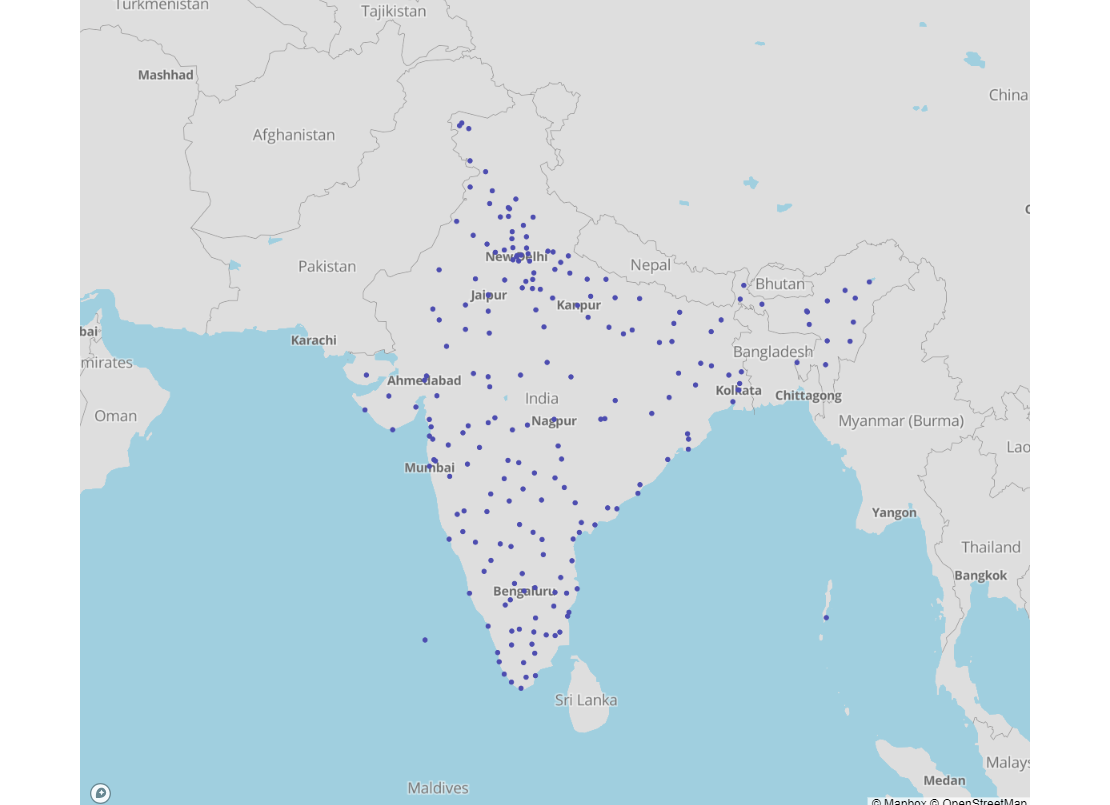
\includegraphics[width=\linewidth]{plot1.png}
  \caption{The plot shows ML powered prediction of where a flood is going to occur, marked by red dots.}
\end{figure}

\begin{figure}[ht]
  \centering
  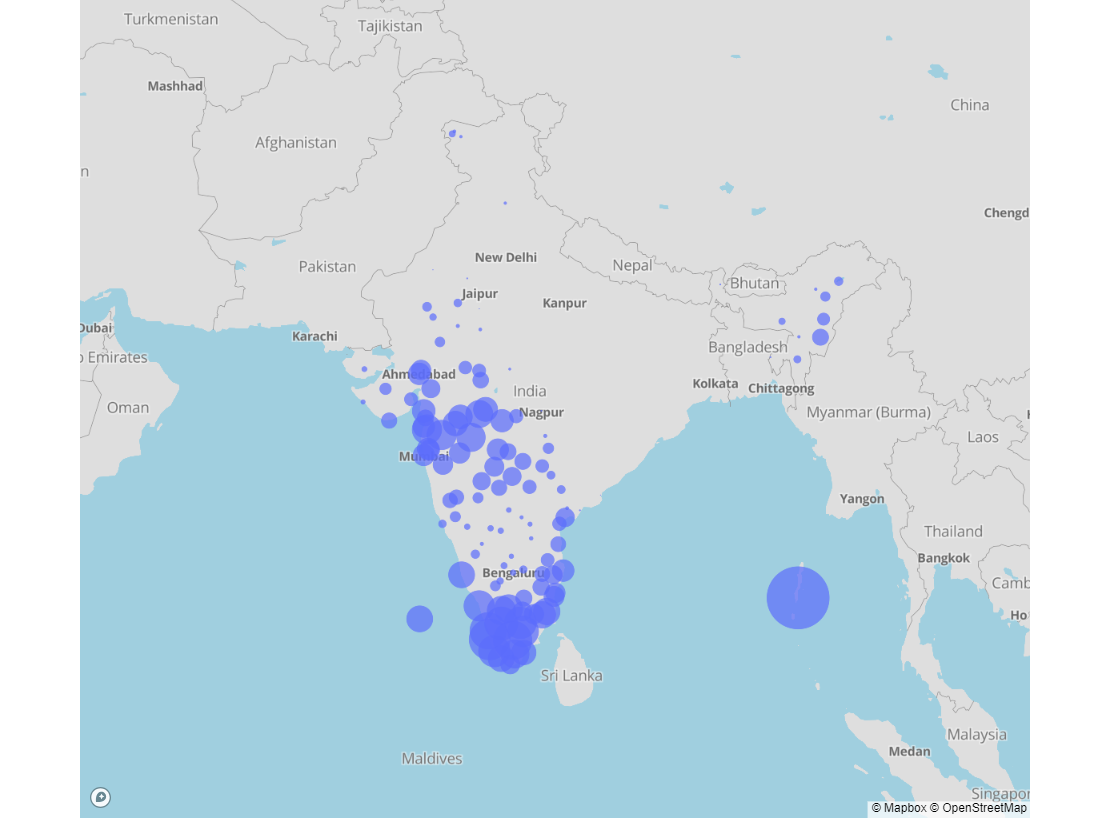
\includegraphics[width=\linewidth]{plot2.png}
  \caption{The plot shows the current precipitation data across the nation. The larger bubbles indicate more precipitation.}
\end{figure}

\begin{figure}[ht]
  \centering
  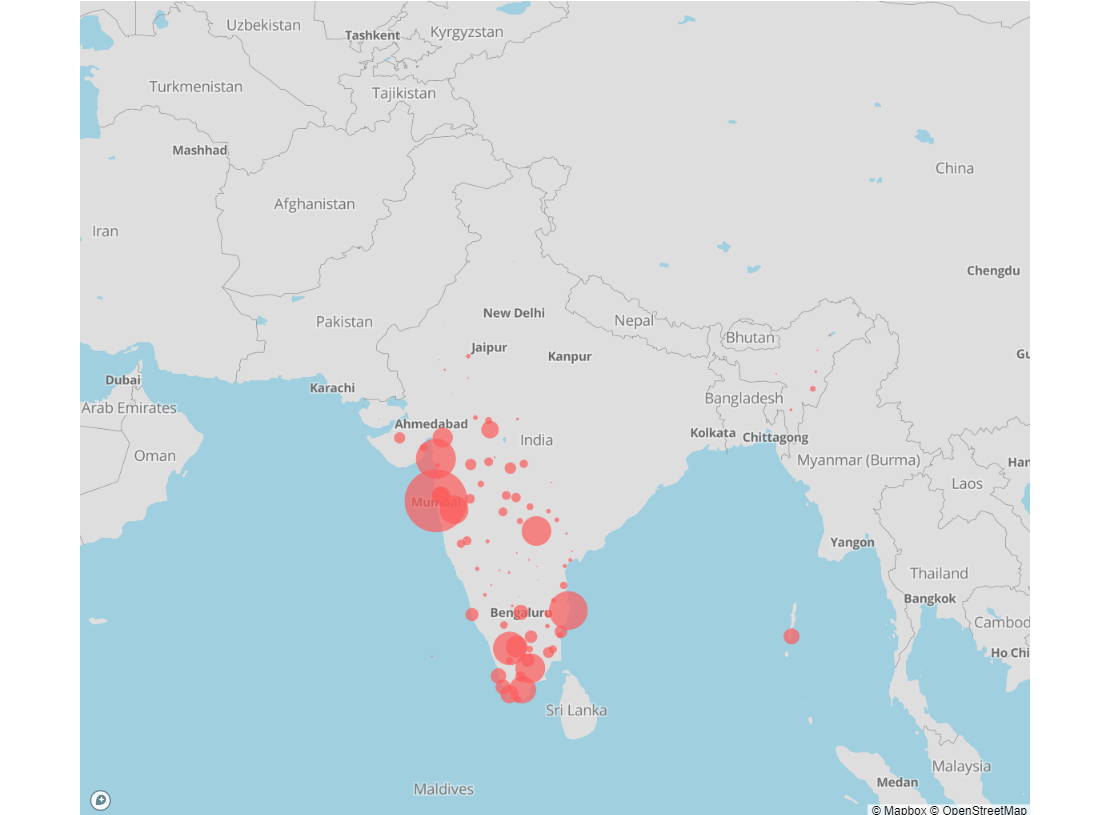
\includegraphics[width=\linewidth]{plot3.png}
  \caption{The plot shows damage analysis, based on the flood risk prediction. The size of the bubbles indicate the extent of predicted damage.}
\end{figure}

\section{Density Maps}

The 3 density maps show flood predictions, damage predictions, and heavy rainfall predictions across India, taking in factors such as precipitation, wind speed, humidity, temperature, cloud cover, as well as previous data history.

\begin{enumerate}
    \item The first plot is my damage analysis plot, which shows a damage analysis, with the colorscale of the density indicating the extent of predicted damage. As shown in Figure 5.4
    \item The second plot is a precipitation plot, showing the forecasted precipitation data across the nation, with the darker areas indicating a greater volume of precipitation.
    \item Lastly, the third plot is a flood prediction plot, which shows my ML-powered prediction of where a flood is most likely to occur given the forecasted environment factors, marked primarily by the darker red spots on a continuous colorbar.
\end{enumerate}

\begin{figure}[ht]
  \centering
  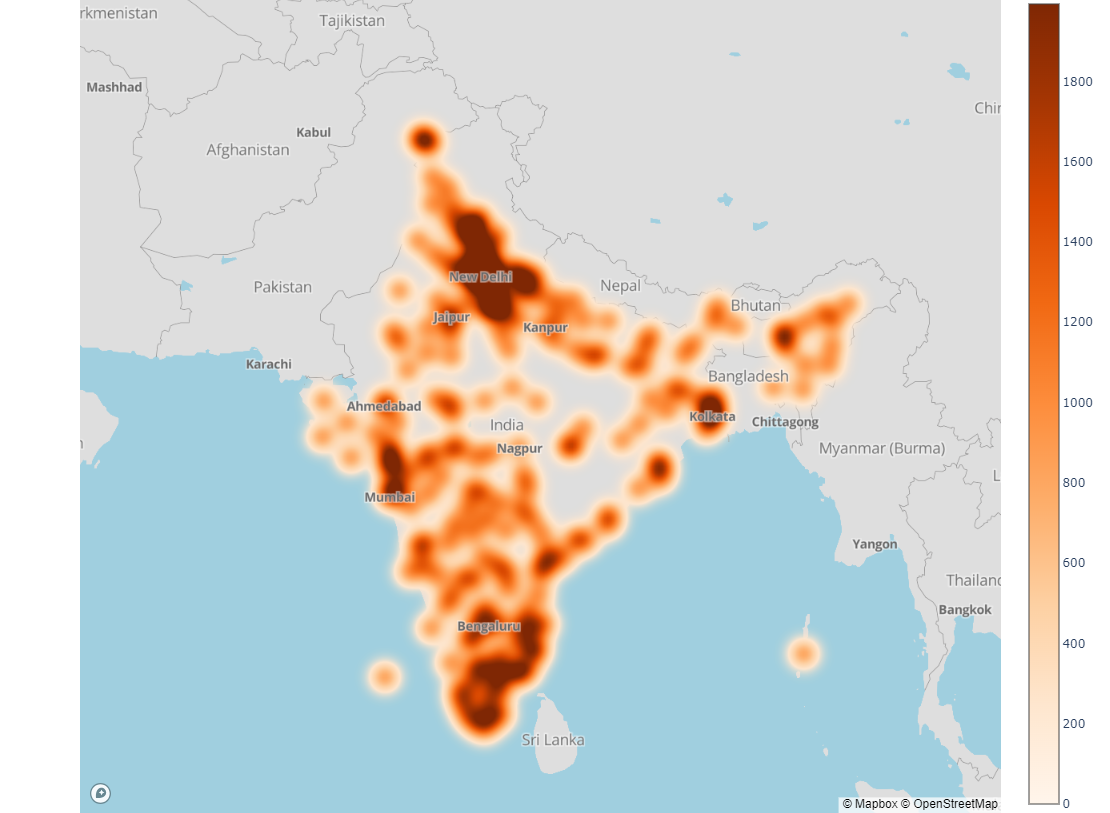
\includegraphics[width=\linewidth]{heatmap1.png}
  \caption{The plot shows damage analysis, based on the flood risk prediction. The colorscale of the density map indicates the extent of predicted damage.}
\end{figure}

\begin{figure}[ht]
  \centering
  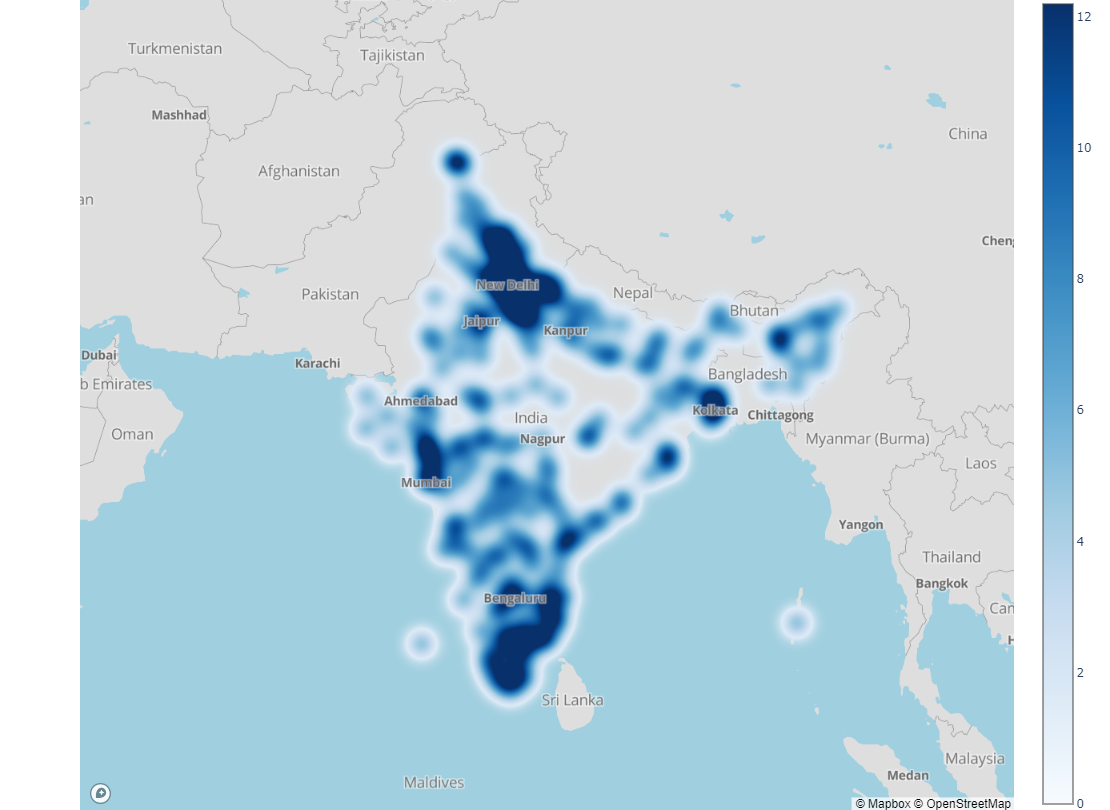
\includegraphics[width=\linewidth]{heatmap2.png}
  \caption{The plot shows the current precipitation data across the nation. The darker areas indicate a greater volume of precipitation.}
\end{figure}

\begin{figure}[ht]
  \centering
  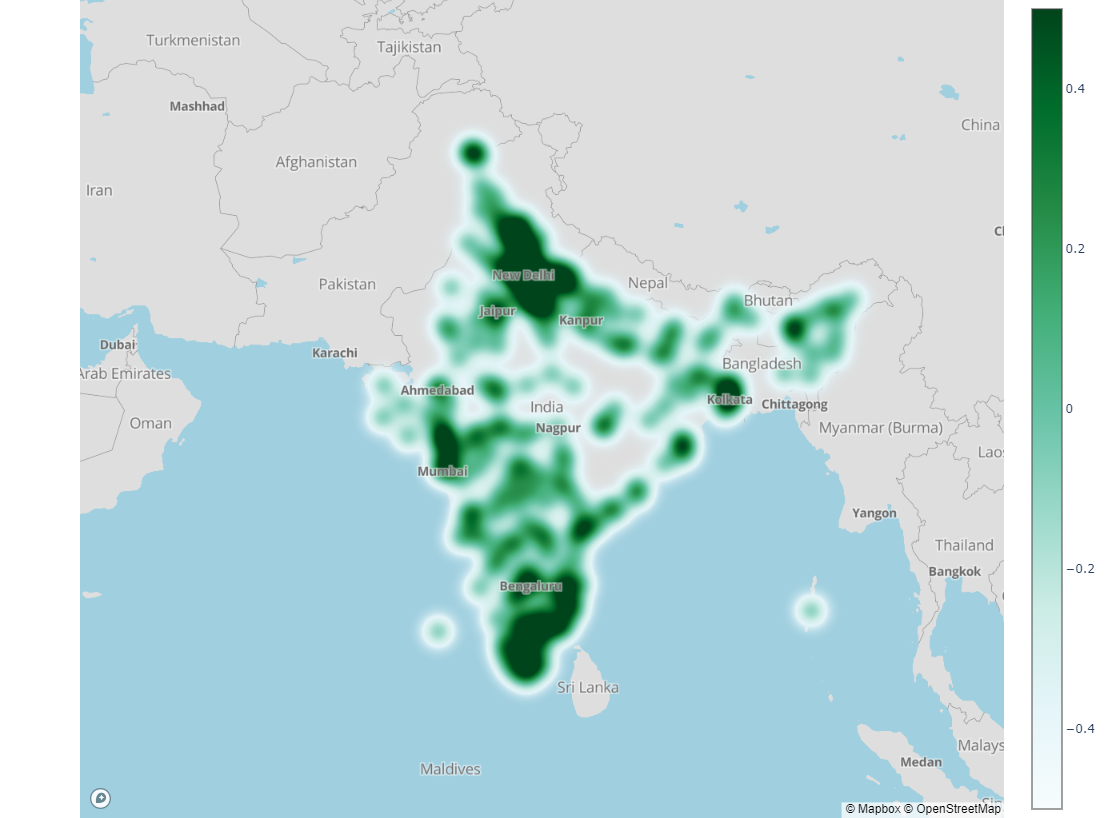
\includegraphics[width=\linewidth]{heatmap3.png}
  \caption{The plot below shows our ML powered prediction of where a flood is most likely to occur given the current environmental factors, marked primarily by the darker spots.}
\end{figure}

\section{Prediction Page}
On predict page, the user simply enters the name of any city in the India. My app then automatically fetches the weather forecast data of that city in realtime, runs this data into my Machine Learning model, and gives instantaneous results, which include the flood prediction, the temperature, the maximum temperature, the humidity, the cloud cover, the windspeed, and the precipitation. As shown in Figure 5.7, 5.8 and 5.9

\begin{figure}[ht]
  \centering
  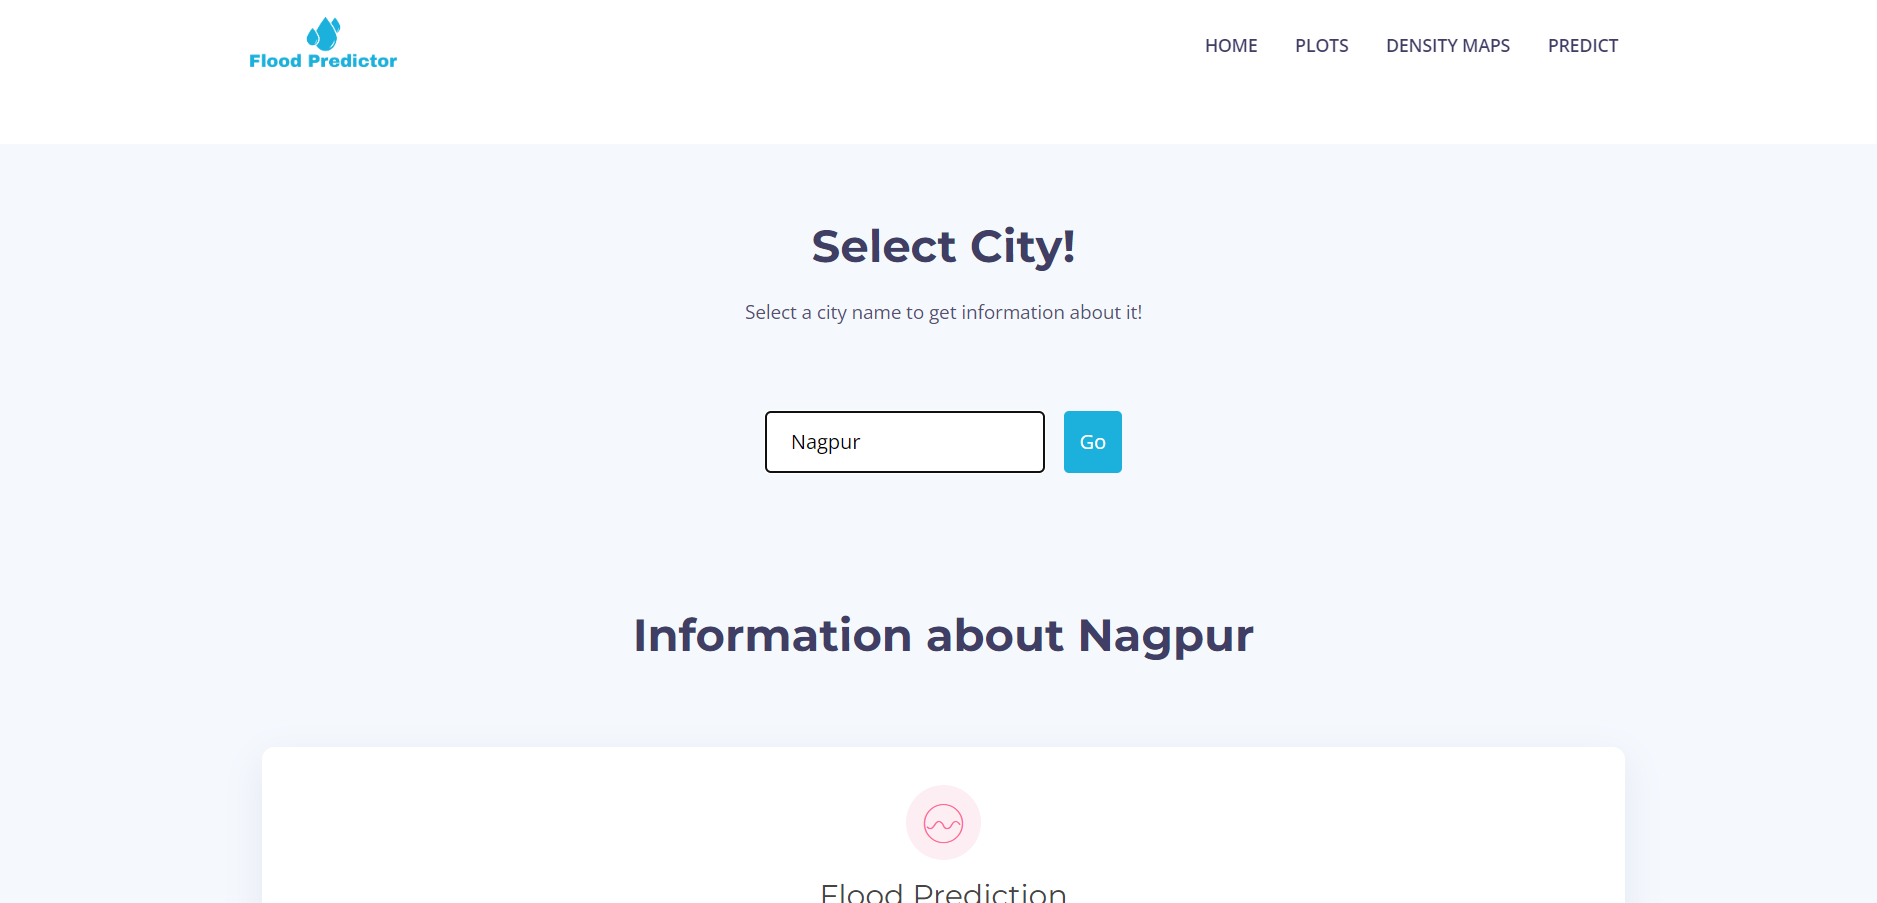
\includegraphics[width=\linewidth]{CityName.png}
  \caption{Prediction page showing user to input any city of India.}
\end{figure}

\begin{figure}[ht]
  \centering
  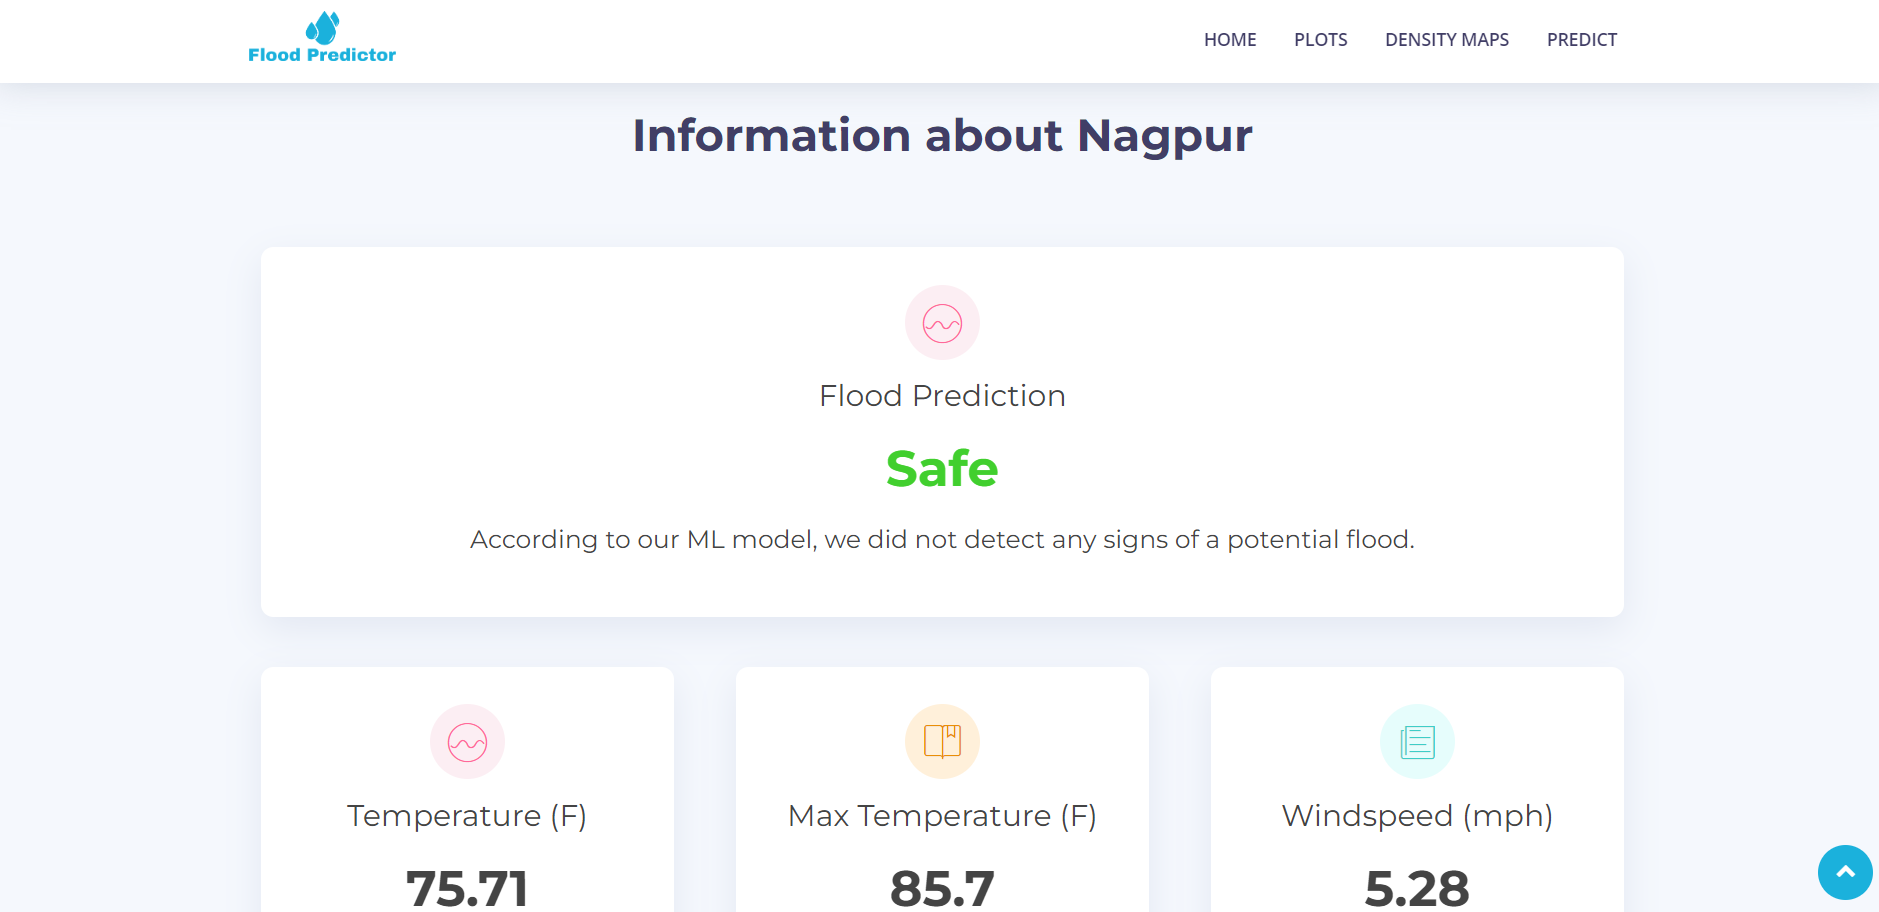
\includegraphics[width=\linewidth]{Predict.png}
  \caption{Based on the Machine Learning model it is showing is city safe.}
\end{figure}

\begin{figure}[ht]
  \centering
  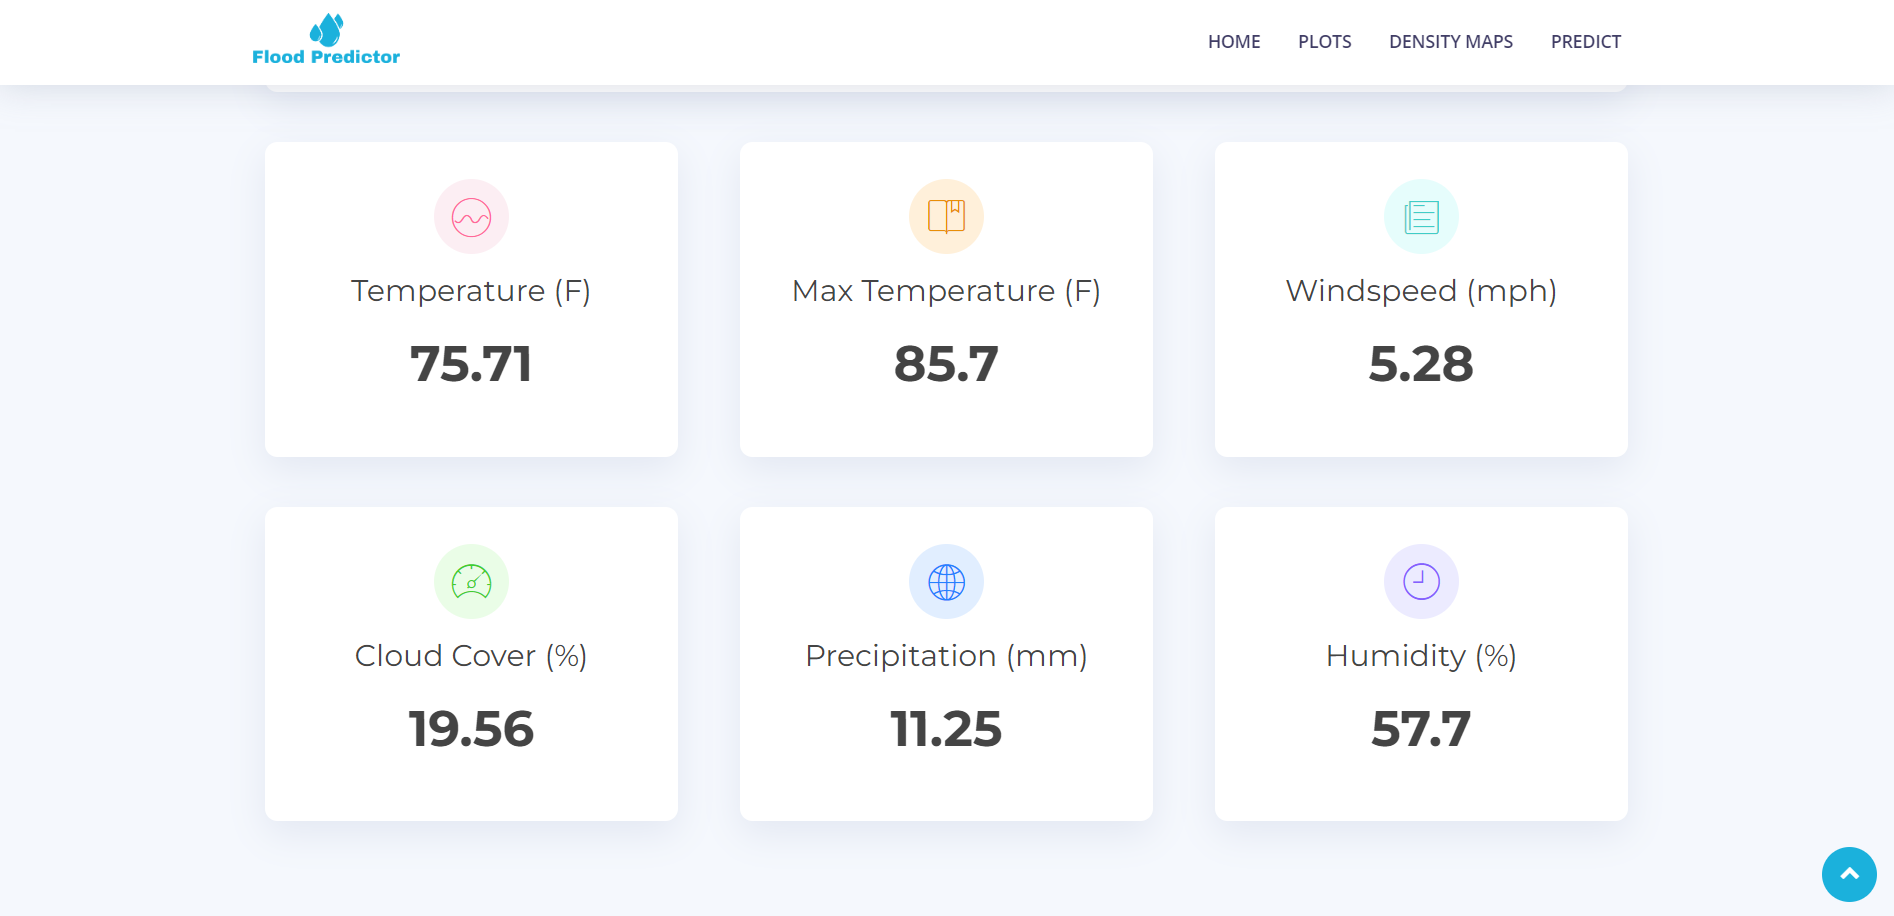
\includegraphics[width=\linewidth]{features.png}
  \caption{Screen showing meteorological data based on which it has done prediction.}
\end{figure}

\chapter{Conclusion}

In conclusion, the development of my project represents a significant stride in addressing the critical issue of floods in India. Through the creation of a web application, equipped with advanced machine learning algorithms, I have successfully implemented a system that predicts future floods based on comprehensive weather forecast data. This endeavor is not just a technological feat; it is a proactive approach to providing users with the tools to better understand and prepare for potential flood risks.

The core components of my project, including plots and heatmaps, offer users a detailed and insightful view of flood predictions, damage estimates, and heavy rainfall forecasts across India. The integration of a user-friendly predict page further enhances accessibility, allowing users to obtain real-time flood predictions for any city worldwide.

The journey to build my project involved overcoming various challenges, most notably the scarcity of available data related to floods in India. Through innovative approaches such as mining flood reports from news sources and utilizing weather APIs, I successfully compiled a diverse dataset. The machine learning model, based on the Random Forest Classifier, demonstrated impressive accuracy, reaching 98.71\% on the test set.

The data visualization aspect of my project, implemented using Plotly chart studio, showcases my commitment to creating detailed, sophisticated, yet comprehensible plots. These visualizations, coupled with the integration of various data augmentation and manipulation techniques, contribute to the effectiveness of my project in conveying critical information.

Throughout this project, I have acquired valuable skills in web scraping, data mining, and data augmentation. Additionally, my foray into Plotly and the exploration of different machine learning models, particularly the Random Forest Classification model, has expanded my technical expertise.

Looking ahead, the vision for my project extends beyond its current scope. I aspire to expand the application globally, covering cities in various countries, and make flood predictions and visualizations accessible worldwide. Furthermore, I recognize the potential of incorporating satellite data for enhanced flood detection and plan to develop an image classification model for this purpose.

In essence, my project is not just a technological achievement but a tool with the potential to make a significant impact on flood preparedness and resource allocation. By providing accurate predictions and valuable insights, this web application stands as a testament to the possibilities of leveraging technology for the greater good, potentially saving lives and safeguarding livelihoods. Visit the live application on \href{https://github.com/SaurabhTiwari4093/Flood-Forecasting}{https://github.com/SaurabhTiwari4093/Flood-Forecasting} or directly on the \href{https://flood-predictor.iccntsd.in}{https://flood-predictor.iccntsd.in} to explore its capabilities and contribute to the ongoing effort to mitigate the impact of floods worldwide.


\chapter{References}
\begin{enumerate}

\item Amazon Web Service: \href{https://aws.amazon.com/}{https://aws.amazon.com/}

\item \href{https://www.ijraset.com/research-paper/flood-prediction-using-machine-learning}{Anil Kumar Ambore, T. Sri Sai Charan, U. Rohit Reddy, T. Samara Simha Reddy, Tarun. G (2023), Flood Prediction using Machine Learning, International Journal for Research in Applied Science \& Engineering Technology (IJRASET) ISSN: 2321-9653; IC Value: 45.98; SJ Impact Factor: 7.538 Volume 11 Issue V May 2023}

\item Beautiful soup 4: \href{https://pypi.org/project/beautifulsoup4/}{https://pypi.org/project/beautifulsoup4/}

\item Flask: \href{https://flask.palletsprojects.com/en/3.0.x/}{https://flask.palletsprojects.com/en/3.0.x/}

\item FloodList: \href{https://floodlist.com/}{https://floodlist.com/}

\item \href{https://www.tandfonline.com/doi/abs/10.1080/02626660209492964}{LIHUA XIONG \& KIERAN M. O'CONNOR (2002) Comparison of four updating models for real-time river flow forecasting, Hydrological Sciences Journal, 47:4, 621-639, DOI: 10.1080/02626660209492964}

\item \href{https://www.mdpi.com/2073-4441/10/11/1536}{Mosavi, A., Ozturk, P., \& Chau, K.-w. (2018). Flood prediction using machine learning models: Literature review. Department of Computer Science (IDI), Norwegian University of Science and Technology (NTNU), NO-7491 Trondheim, Norway; Department of Civil and Environmental Engineering, Hong Kong Polytechnic University, Hong Kong, China; dr.kwok-wing.chau@polyu.edu.hk. Correspondence: amir.mosavi@ntnu.no (A.M.); pinar@ntnu.no (P.O.). Received: 1 September 2018; Accepted: 17 October 2018; Published: 27 October 2018.}

\item \href{https://hess.copernicus.org/articles/26/4013/2022/}{Nevo, S., Morin, E., Rosenthal, A. G., Metzger, A., Barshai, C., Weitzner, D., ... Matias, Y. (2023). Flood forecasting with machine learning models in an operational framework. Google Research, Yigal Alon 96, Tel-Aviv 6789141, Israel; Hebrew University of Jerusalem, Safra Campus, Jerusalem 91904, Israel.}

\item Plotly chart studio: \href{https://chart-studio.plotly.com/}{https://chart-studio.plotly.com/}

\item Python: \href{https://www.python.org/}{https://www.python.org/}

\item Population Data: \href{https://public.opendatasoft.com/}{https://public.opendatasoft.com/}

\item Weather Data \& API Global Forecast \& History Data: \href{https://www.visualcrossing.com/}{https://www.visualcrossing.com/}

\end{enumerate}

\chapter{Appendices}

\section{Python code for data collection and mining}

\subsection{scraper.py}

\begin{lstlisting}
import requests
import datetime

def get_data(date, month, year, days, location):
    a = datetime.date(year, month, date)
    b = a - datetime.timedelta(days)
    
    k = "https://weather.visualcrossing.com/VisualCrossingWebServices/
    rest/services/weatherdata/history?&aggregateHours=" + str(24 * days) + "&startDateTime=" + str(b) + "T00:00:00&endDateTime=" + str(a) + "T00:00:00&unitGroup=uk&contentType=json&dayStartTime=0:0:00&
    dayEndTime=0:0:00&location=" + location + ",India&key=XHWV4W6GK29MQK6J9BBM2GNKC"
    x = requests.get(k).json()['locations']
    
    for i in x:
        y = x[i]

    y = y['values'][0]
    final = [y['temp'], y['maxt'], y['wspd'], y['cloudcover'], y['precip'], y['humidity'], y['precipcover']]

    return final

states = ['Karnataka', 'Gujarat', 'Rajasthan', 'Maharashtra', 'Madhya Pradesh']
import csv
import random
f = open('data1.csv', mode='w', newline = '')
writer = csv.writer(f, delimiter=',')

for i in states:
    for j in range(1, 31):
        a = random.randint(1, 28)
        b = random.randint(1, 12)
        c = random.randint(2013, 2019)

        k = get_data(a, b, c, 15, i)

        if k[4] != None:
            if k[4] < 20:
                print(k)
                print(j)
                writer.writerow(k + [0])

def extract_date(x):
    k = x.split(" ")

    a = int(k[0])

    d = {'january':1, 'february':2, 'march':3, 'april':4, 'may':5, 'june':6, 'july':7, 'august':8, 'september':9, 'october':10, 'november':11, 'december':12}
    b = d[k[1][0:len(k[1]) - 1].lower()]

    c = int(k[2])

    return [a, b, c]

def process(k):
    x = extract_date(k[1])

    return get_data(x[0], x[1], x[2], 15, k[0])

f = open('data.csv', mode='w', newline = '')
writer = csv.writer(f, delimiter=',')

with open('mined.csv', mode='r') as csv_file:
    csv_reader = csv.reader(csv_file)
    
    for row in csv_reader:
        print(row)
        
        writer.writerow(process(row) + [1])
\end{lstlisting}

\subsection{get\_forecast.py}
\begin{lstlisting}
import csv
import requests

def get_data(lat, lon):

    k = "https://weather.visualcrossing.com/VisualCrossingWebServices/
    rest/services/weatherdata/forecast?locations=" + \
        str(lat) + "%2C%20" + str(lon) + \
        "&aggregateHours=24&unitGroup=us&shortColumnNames=false&
        contentType=json&key=XHWV4W6GK29MQK6J9BBM2GNKC"
    x = requests.get(k).json()['locations']
    for i in x:
        y = x[i]['values']

    final = [0, 0, 0, 0, 0, 0]

    for j in y:
        final[0] += j['temp']
        if j['maxt'] > final[1]:
            final[1] = j['maxt']
        final[2] += j['wspd']
        final[3] += j['cloudcover']
        final[4] += j['precip']
        final[5] += j['humidity']
    final[0] /= 15
    final[2] /= 15
    final[3] /= 15
    final[5] /= 15

    return final

def testConnection():
    return "yo"

f = open('cities.csv', 'r', encoding='UTF-8')
ff = open('plotting.csv', mode='w', newline='')
writer = csv.writer(ff, delimiter=',')

r = csv.reader(f)

for row in r:
    print(row)
    writer.writerow(get_data(row[1], row[2]))   
\end{lstlisting}

\subsection{data\_augment.py}
\begin{lstlisting}
import csv
import random 

def augment(k):
    final = []
    for i in range(0, 7):
        final.append(round(random.uniform(33.33, 66.66), 2) + float(k[i]))

    return final + [int(k[7])]

data1 = open('data.csv', mode='r')
data0 = open('data1.csv', mode='r')

reader1 = csv.reader(data1)

reader0 = csv.reader(data0)

f = open('final_data.csv', mode='w', newline = '')
writer = csv.writer(f, delimiter=',')

for row1 in reader1:
    writer.writerow(row1)
    for i in range(0, 19):
        writer.writerow(augment(row1))

for row0 in reader0:
    writer.writerow(row0)
    for i in range(0, 19):
        writer.writerow(augment(row0))
\end{lstlisting}

\section{Python code for Machine Learning model training}

\begin{lstlisting}
import pandas as pd
from sklearn.model_selection import train_test_split
from sklearn.metrics import accuracy_score
from sklearn.ensemble import RandomForestClassifier
import pickle

data = pd.read_csv("final_data.csv")
y = data['class']
X = data.drop('class', axis=1)
X_train, X_test, y_train, y_test = train_test_split(X, y,test_size=0.2)

classifier = RandomForestClassifier(n_estimators = 50, criterion = 'entropy', random_state = 0)

classifier.fit(X_train, y_train)

pred = classifier.predict(X_test)
accuracy = accuracy_score(y_test, pred)

print("accuracy: " + str(accuracy * 100) + "%")

pickle.dump(classifier, open('model.pickle', 'wb'))   
\end{lstlisting}

\section{Python code for data visualization and plotting}

\subsection{generate\_plotting\_data.py}

\begin{lstlisting}
import csv
import pickle

model = pickle.load(open('model.pickle', 'rb'))
c = open('cities.csv', 'r', encoding='UTF-8')

cr = csv.reader(c)

cities = []

for c_row in cr:
    cities.append(c_row) 

d = open('plotting.csv', 'r', encoding='UTF-8')

dr = csv.reader(d)

forecast = []
for d_row in dr:
    k = list(map(float, d_row))
    forecast.append([k[4], model.predict([k])[0]])

ff = open('final_plot.csv', mode='w', newline = '', encoding="UTF-8")
writer = csv.writer(ff, delimiter=',')

for i in range(0, len(forecast)):
    writer.writerow(cities[i] + forecast[i])
print(forecast)    
\end{lstlisting}

\subsection{population\_gen.py}

\begin{lstlisting}
import requests
import json
import csv

population_data = []

def get_city_opendata(city, country):
    tmp = 'https://public.opendatasoft.com/api/explore/v2.1/catalog/
    datasets/geonames-all-cities-with-a-population-500/
    records?refine=country:%s&refine=ascii_name:%s'
    cmd = tmp % (country, city)
    res = requests.get(cmd)
    dct = json.loads(res.content)
    out = dct['results'][0]['population']
    return out

csv_file = "finalfinal.csv"

with open(csv_file, 'r') as f:
    reader = csv.reader(f)
    header = next(reader)
    header.append("population")  # Add "pop" to the existing header

    for row in reader:
        if row[0] != "city":
            try:
                pop = get_city_opendata(row[0], 'India')
                row.append(pop)
                population_data.append(row)
            except:
                print("error in", row[0])
                row.append(0)
                population_data.append(row)

with open('finalfinal.csv', 'w', newline='') as f:
    writer = csv.writer(f)
    writer.writerow(header)  # Write the updated header
    for row in population_data:
        writer.writerow(row)

# Also corrected some cities spelling and manually added population
\end{lstlisting}

\subsection{pop\_multiply\_precip.py}

\begin{lstlisting}
import csv

csv_file = "finalfinal.csv"

rows = []

with open(csv_file, 'r') as f:
    reader = csv.reader(f)
    header = next(reader)  # Read the header row
    header.append("damage")  # Add a new column header

    for row in reader:
        if row[0] != "city":
            dam = round(float(row[3]) * float(row[5])/10000, 2)
            row.append(dam)
        rows.append(row)

with open('finalfinal.csv', 'w', newline='') as f:
    writer = csv.writer(f)
    writer.writerow(header)  # Write the modified header
    writer.writerows(rows)  # Write the modified rows
   
\end{lstlisting}

\section{Python code prediction of flood}

\begin{lstlisting}
import requests

def get_data(lat, lon):

    k = "https://weather.visualcrossing.com/VisualCrossingWebServices/
    \rest/services/weatherdata/forecast?locations=" + str(lat) + "%2C%20" + str(lon)+"&aggregateHours=24&unitGroup=us&
    shortColumnNames=false&contentType=json&
    key=XHWV4W6GK29MQK6J9BBM2GNKC"
    x = requests.get(k).json()['locations']

    for i in x:
        y = x[i]['values']

    final = [0, 0, 0, 0, 0, 0]

    for j in y:
        final[0] += j['temp']
        if j['maxt'] > final[1]:
            final[1] = j['maxt']
        final[2] += j['wspd']
        final[3] += j['cloudcover']
        final[4] += j['precip']
        final[5] += j['humidity']
    final[0] /= 15
    final[2] /= 15
    final[3] /= 15
    final[5] /= 15
    
    return final

def testConnection():
    return "yo"    
\end{lstlisting}

\section{Flask code to connect Frontend \& ML Model Pickel}

\begin{lstlisting}
import flask
from flask import render_template, request

import pickle
from training import prediction
import requests
application = flask.Flask(__name__)

model = pickle.load(open("model.pickle", 'rb'))

@application.route("/")
@application.route('/index.html')
def index() -> str:
    """Base page."""
    return flask.render_template("index.html")

@application.route('/plots.html')
def plots():
    return render_template('plots.html')

@application.route('/densityMaps.html')
def heatmaps():
    return render_template('densityMaps.html')

@application.route('/predicts.html')
def predicts():
    return render_template('predicts.html', cityname="Information about the city")

@application.route('/predicts.html', methods=["GET", "POST"])
def get_predicts():
    try:
        cityname = request.form["city"]
        # print(cityname)
        URL = "https://geocode.search.hereapi.com/v1/geocode"
        location = cityname
        # Acquire from developer.here.com
        api_key = 'ftKvGdH2ItSBc6N3Jbh4TzpH6F57uHHqw4Us4Uoj0HM'
        PARAMS = {'apikey': api_key, 'q': location}
        # sending get request and saving the response as response object
        r = requests.get(url=URL, params=PARAMS)
        data = r.json()
        latitude = data['items'][0]['position']['lat']
        longitude = data['items'][0]['position']['lng']
        final = prediction.get_data(latitude, longitude)

        final[4] *= 15
        if str(model.predict([final])[0]) == "0":
            pred = "Safe"
        else:
            pred = "Unsafe"

        return render_template('predicts.html', cityname="Information about " + cityname, temp=round(final[0], 2), maxt=round(final[1], 2), wspd=round(final[2], 2), cloudcover=round(final[3], 2), percip=round(final[4], 2), humidity=round(final[5], 2), pred=pred)
    except:
        return render_template('predicts.html', cityname="Oops, we weren't able to retrieve data for that city.")

if __name__ == "__main__":
    application.run(debug=True)
\end{lstlisting}

\section{Run code in local machine}
\begin{enumerate}
\item Clone the project from \href{https://github.com/SaurabhTiwari4093/Flood-Forecasting}{https://github.com/SaurabhTiwari4093/Flood-Forecasting}
\item Activate virtual environment
\item run pip install -r requirements.txt
\item run python application.py
\item You're Done!
\end{enumerate}





\end{document}
